\documentclass[twocolumn]{aastex63}

\newcommand{\vdag}{(v)^\dagger}
\newcommand\aastex{AAS\TeX}
\newcommand\latex{L\textsubscript{E}\TeX}

\shorttitle{A One-parameter, Purely Baryon Driven, Dark Matter Density Profile}
\shorttitle{Galactic Rotation Curves from a Singular Parameter}
\shortauthors{Thomas C. Andersen}
\graphicspath{{../sparc/power-59W}{../sparc/power-59W/curves}}

\begin{document}

\title{A One-parameter, Purely Baryon Driven, Dark Matter Density Profile}

\author[0000-0003-1614-4124]{Thomas C. Andersen}
\affiliation{nSCIr \\
Ontario, Canada}

\begin{abstract}
We present a novel empirical equation for the dark matter derived only from galactic (gas) kinematics. It is defined simply and entirely by the one-parameter scaling relation $\rho_{\text{dm}} = P/c^3 \cdot n_b^{2/3}$, where $n_b$ is the local volumetric baryon density and $P$ is a universal global constant in units of power. To evaluate its applicability, we optimize and test this relation against the complete Spitzer Photometry and Accurate Rotation Curves (SPARC) database, with over 3000 data points across 175 morphologically diverse galaxies. The combination of $P$ and the  $2/3$ scaling law of dark mass density results in dark mass starting to be substantial when baryons are about a millimetre apart. The model is easily testable, as it has one free parameter and offers predictions at all scales.   
\end{abstract}

\keywords{Dark matter, Dark mass, SPARC, Rotation curves}

\section{Introduction} \label{sec:intro}

\subsection{History} \label{subsec:history}

For over four decades, the standard cosmological paradigm ($\Lambda$CDM) has successfully explained large-scale structure formation, cosmic microwave background anisotropies, and cosmic shear observations by invoking a dominant component of cold dark matter. However, at galactic and sub-galactic scales, the nature of this missing mass field remains one of the most persistent crises in modern physics. Despite intensive efforts spanning astronomical observations, deep underground direct-detection experiments, and high-energy collider searches, particle dark matter candidates---ranging from Weakly Interacting Massive Particles (WIMPs) to ultra-light axions---have eluded detection across nearly thirty orders of magnitude in predicted mass scales. Even assuming a (perhaps undetectable) particle like dark matter, problems persist. For example, modelling the dark matter distribution in galaxies, where Sancisi's Law\citep{sancisiVisibleMatterDark2004} \citep{lelliSPARCMassModels2016}, \citep{Lelli2017}and the puzzling excellent performance of the MOND framework indicate that a conventional particle dark matter model may never work. 

\subsection{Current Approaches} \label{subsec:current}
There are currently two primary paths of investigation in galactic dynamics. The first relies on multi-parameter empirical density profiles, such as the Navarro-Frenk-White (NFW)\citep{navarroUniversalDensityProfile1997} or Burkert profiles\citep{burkertStructureDarkMatter1995}, which are fitted to individual galactic rotation curves. While these profiles effectively capture kinematic features, they generally treat parameters like scale radius ($r_s$) and central density ($\rho_0$) as free, independent variables unique to each galaxy. This introduces a large parameter space that requires individual, galaxy-by-galaxy 'tuning.' The second path, Modified Newtonian Dynamics (MOND), abandons the dark matter hypothesis entirely, accounting for anomalous galactic rotation curves by introducing a universal acceleration constant ($a_0 \approx 1.2 \times 10^{-10} \text{ m s}^{-2}$) below which Newtonian gravity breaks down. MOND's striking empirical success, particularly in explaining the Radial Acceleration Relation (RAR) and the Baryonic Tully-Fisher Relation (BTFR)\citep{Lelli2017}, demonstrates that galactic kinematics are deeply coupled to the distribution of baryonic matter.

\subsection{Our Model} \label{subsec:ourmodel}
Rather than approaching this problem from the bottom up by inventing novel particle physics models or modifying gravitational field equations, this paper approaches the dark mass problem from the opposite direction: top-down phenomenological mapping. Historically, when fundamental microphysics are unknown, progress is driven by identifying the exact geometric and empirical laws mandated by observation - much as Kepler's laws mapping planetary orbits paved the structural path for Newton's universal gravitation. Thus, we avoid investigating the 'why' of our dark matter model here. 

In this work, we propose a one-parameter empirical dark matter density profile governed by a universal geometric scaling relation: $\rho_{\text{dm}} = K \cdot n_b^{2/3}$, where $n_b$ is the local volumetric baryon density and $K$ is our new universal constant. By utilizing the complete, high-fidelity Spitzer Photometry and Accurate Rotation Curves (SPARC) database as a benchmark, we bypass individual halo tuning entirely. We test whether this singular, invariant scaling law can reproduce observed galactic rotation curves across all 175 SPARC galaxies. 

The $2/3$ exponent is what sets this model apart. With our value for $P$, a gas with a baryonic number density of $10^{-5}\ baryons/cm^3$ would mean a dark matter density of almost 1000 times heavier that of the gas itself, while at $100 baryons/cm^3$ the dark mass only adds about $30\%$ to the density of the gas. By (galactic) observation, we surmise that this dark mass  has a negligible effect on individual particle dynamics. We stay away from speculating on the exact micro dynamics of this 'dark mass' field, instead modelling the field from the data.   

\section{Data and Methodology} \label{sec:meth}

\subsection{The Universal Scaling Model}
The local dark matter density ($\rho_{\text{dm}}$) is assumed to follow a geometric power-law relation:
\begin{equation}
\rho_{\text{dm}} = P/c^3 \cdot n_b^{2/3},
\end{equation}
where $n_b$ represents the local volumetric baryon density (calculated here from the raw SPARC neutral hydrogen gas profiles), and $P$ is a universal invariant constant across all systems, determined by a best fit to the SPARC data.  Our best fit of the parameter $P$ is: 

\begin{equation}
P \approx 59\ Watts.
\end{equation}


\subsection{Statistical Optimization via Least Absolute Deviations (LAD)}
Because galactic rotation curve data points exhibit localized spatial dependencies (e.g., radial proximity within individual galaxies sharing systematic streaming motions or beam smearing), traditional ordinary least squares ($\chi^2$) approaches can be disproportionately skewed by local outliers. We instead evaluate the goodness-of-fit using the Least Absolute Deviations (LAD) framework. 

The global model parameters are optimized by directly minimizing the total absolute residual sum of the observed ($V_{\text{obs}}$) and predicted ($V_{\text{pred}}$) rotation velocities across the entire ensemble of $N = 3,391$ data points:
\begin{equation}
\text{Total LAD} = \sum_{i=1}^{N} |V_{\text{obs}, i} - V_{\text{pred}, i}|
\end{equation}
The resulting model fit is characterized via the Mean Absolute Error (MAE), defined as $\text{MAE} = \text{Total LAD} / N$, providing a, velocity-space measure of global model precision in units of km/s.

\section{Python code description} \label{sec:python}
The raw data is read in from the SPARC website publically availble data, blah blah

\section{Results} \label{sec:results}


\section{Discussion} \label{sec:discussion}
\subsection{Newtonian Dynamics}

\begin{figure}[ht!]
\centering
\label{fig:example fits}
\begin{center}

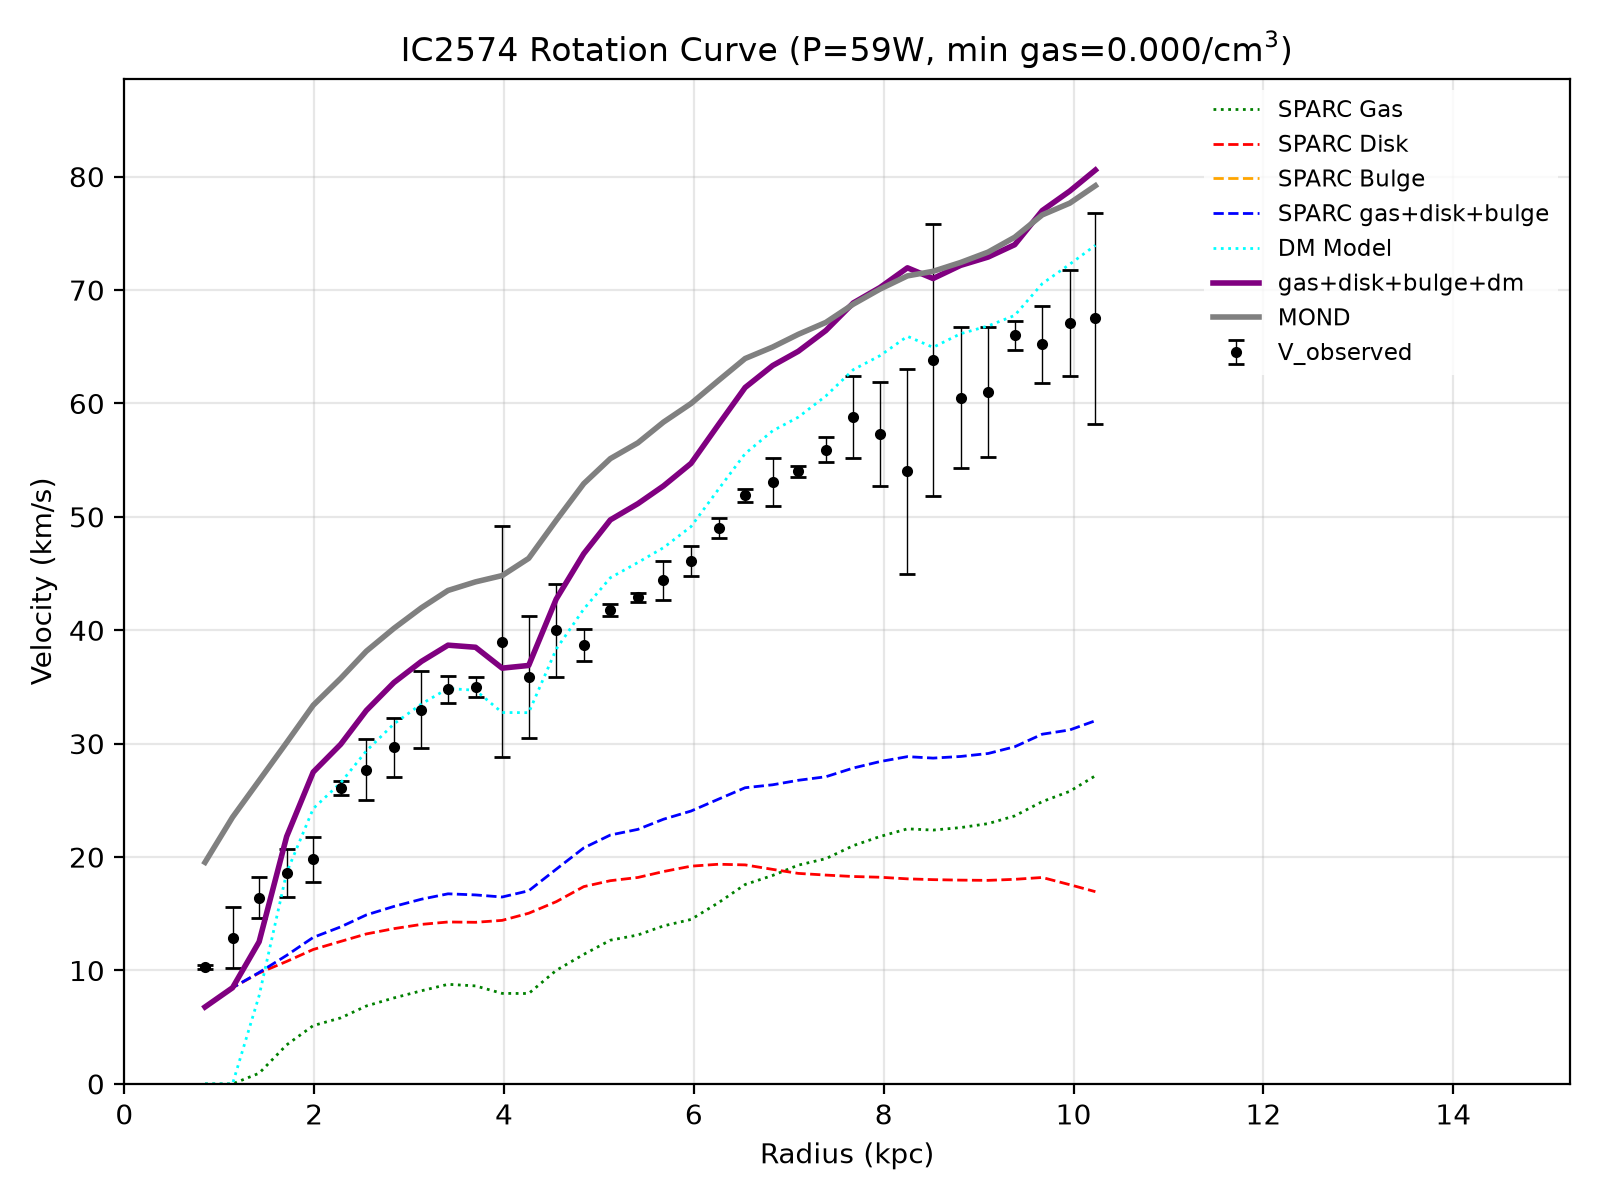
\includegraphics[width=0.48\textwidth]{IC2574-power-59W.png} 
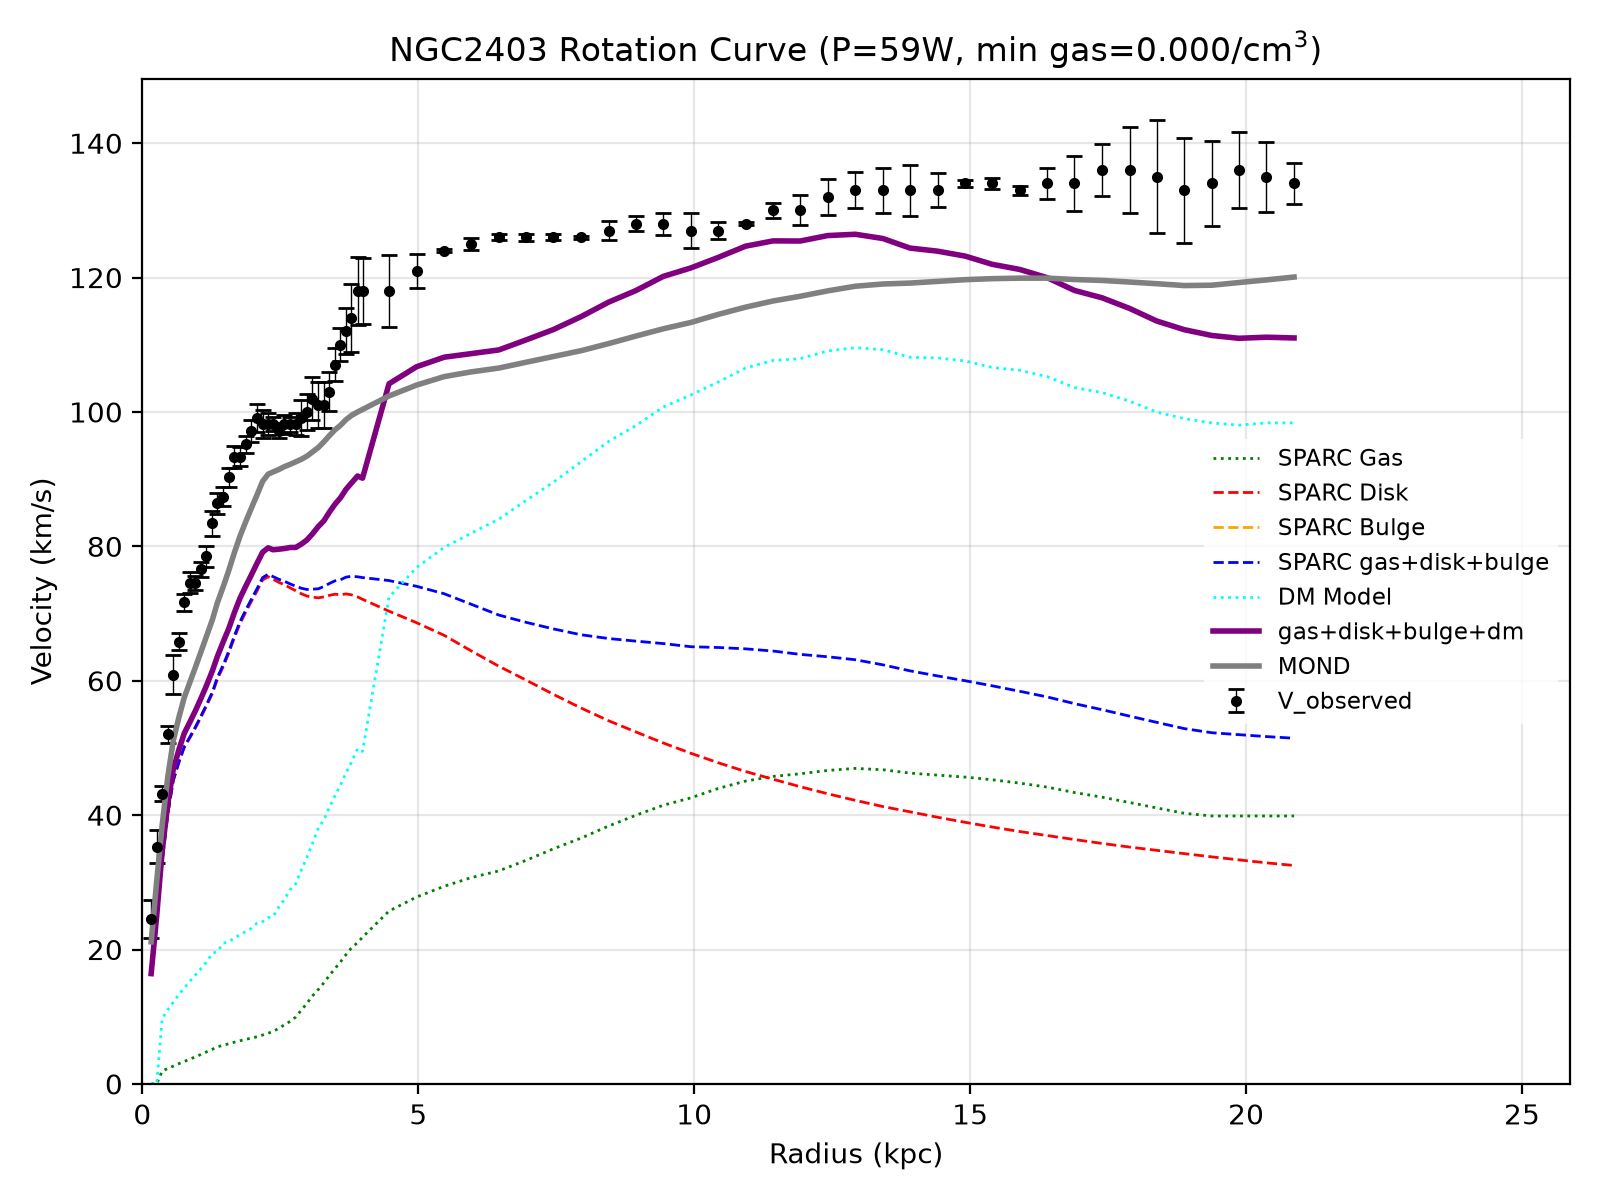
\includegraphics[width=0.48\textwidth]{NGC2403-power-59W.png} 
\end{center}
\caption{Example fits. The only fit parameter 'P' is fixed for all 175 galaxies once it is determined. The purple line shows the total fit by this model. All 175 images are available online. Renzo's rule is honoured at 4 kpc in the IC2574 plot, and at 2 - 5kpc in the NGC 2403 plot.}
\end{figure}



\begin{figure}[ht!]
\centering
\label{fig:newton}
\begin{center}

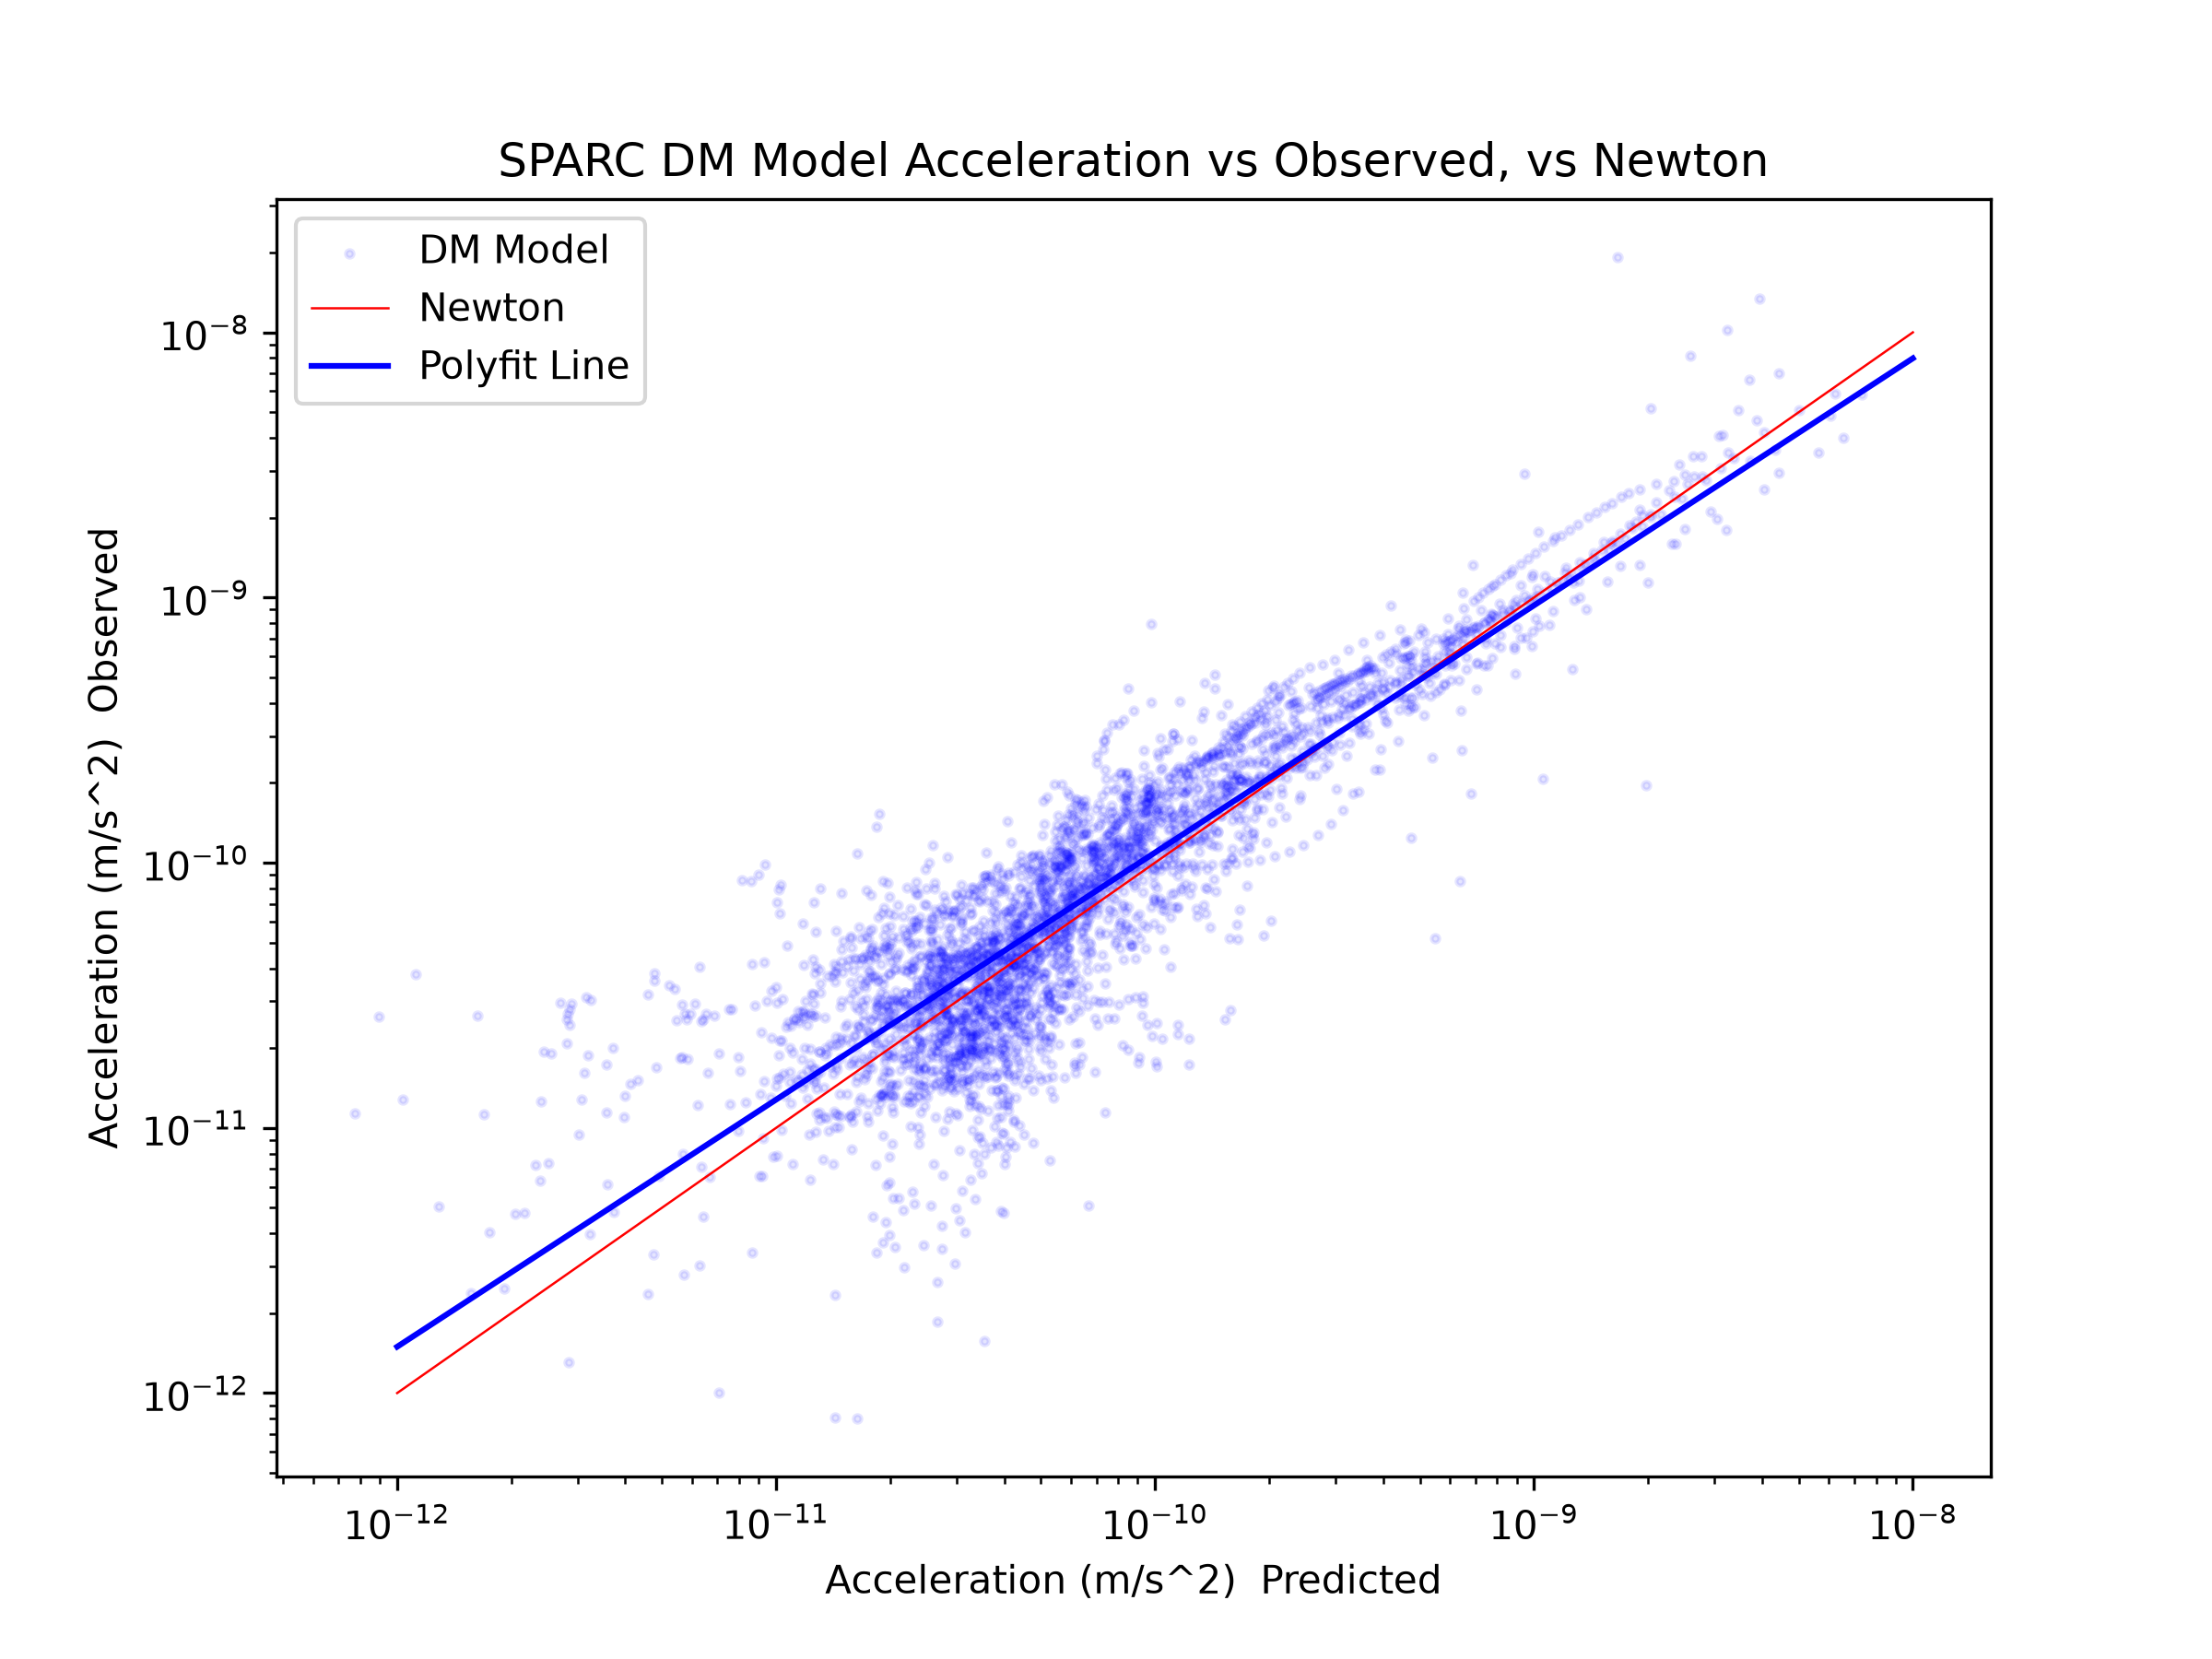
\includegraphics[width=0.48\textwidth]{acceleration_scatter_combined-power-59W.png} 
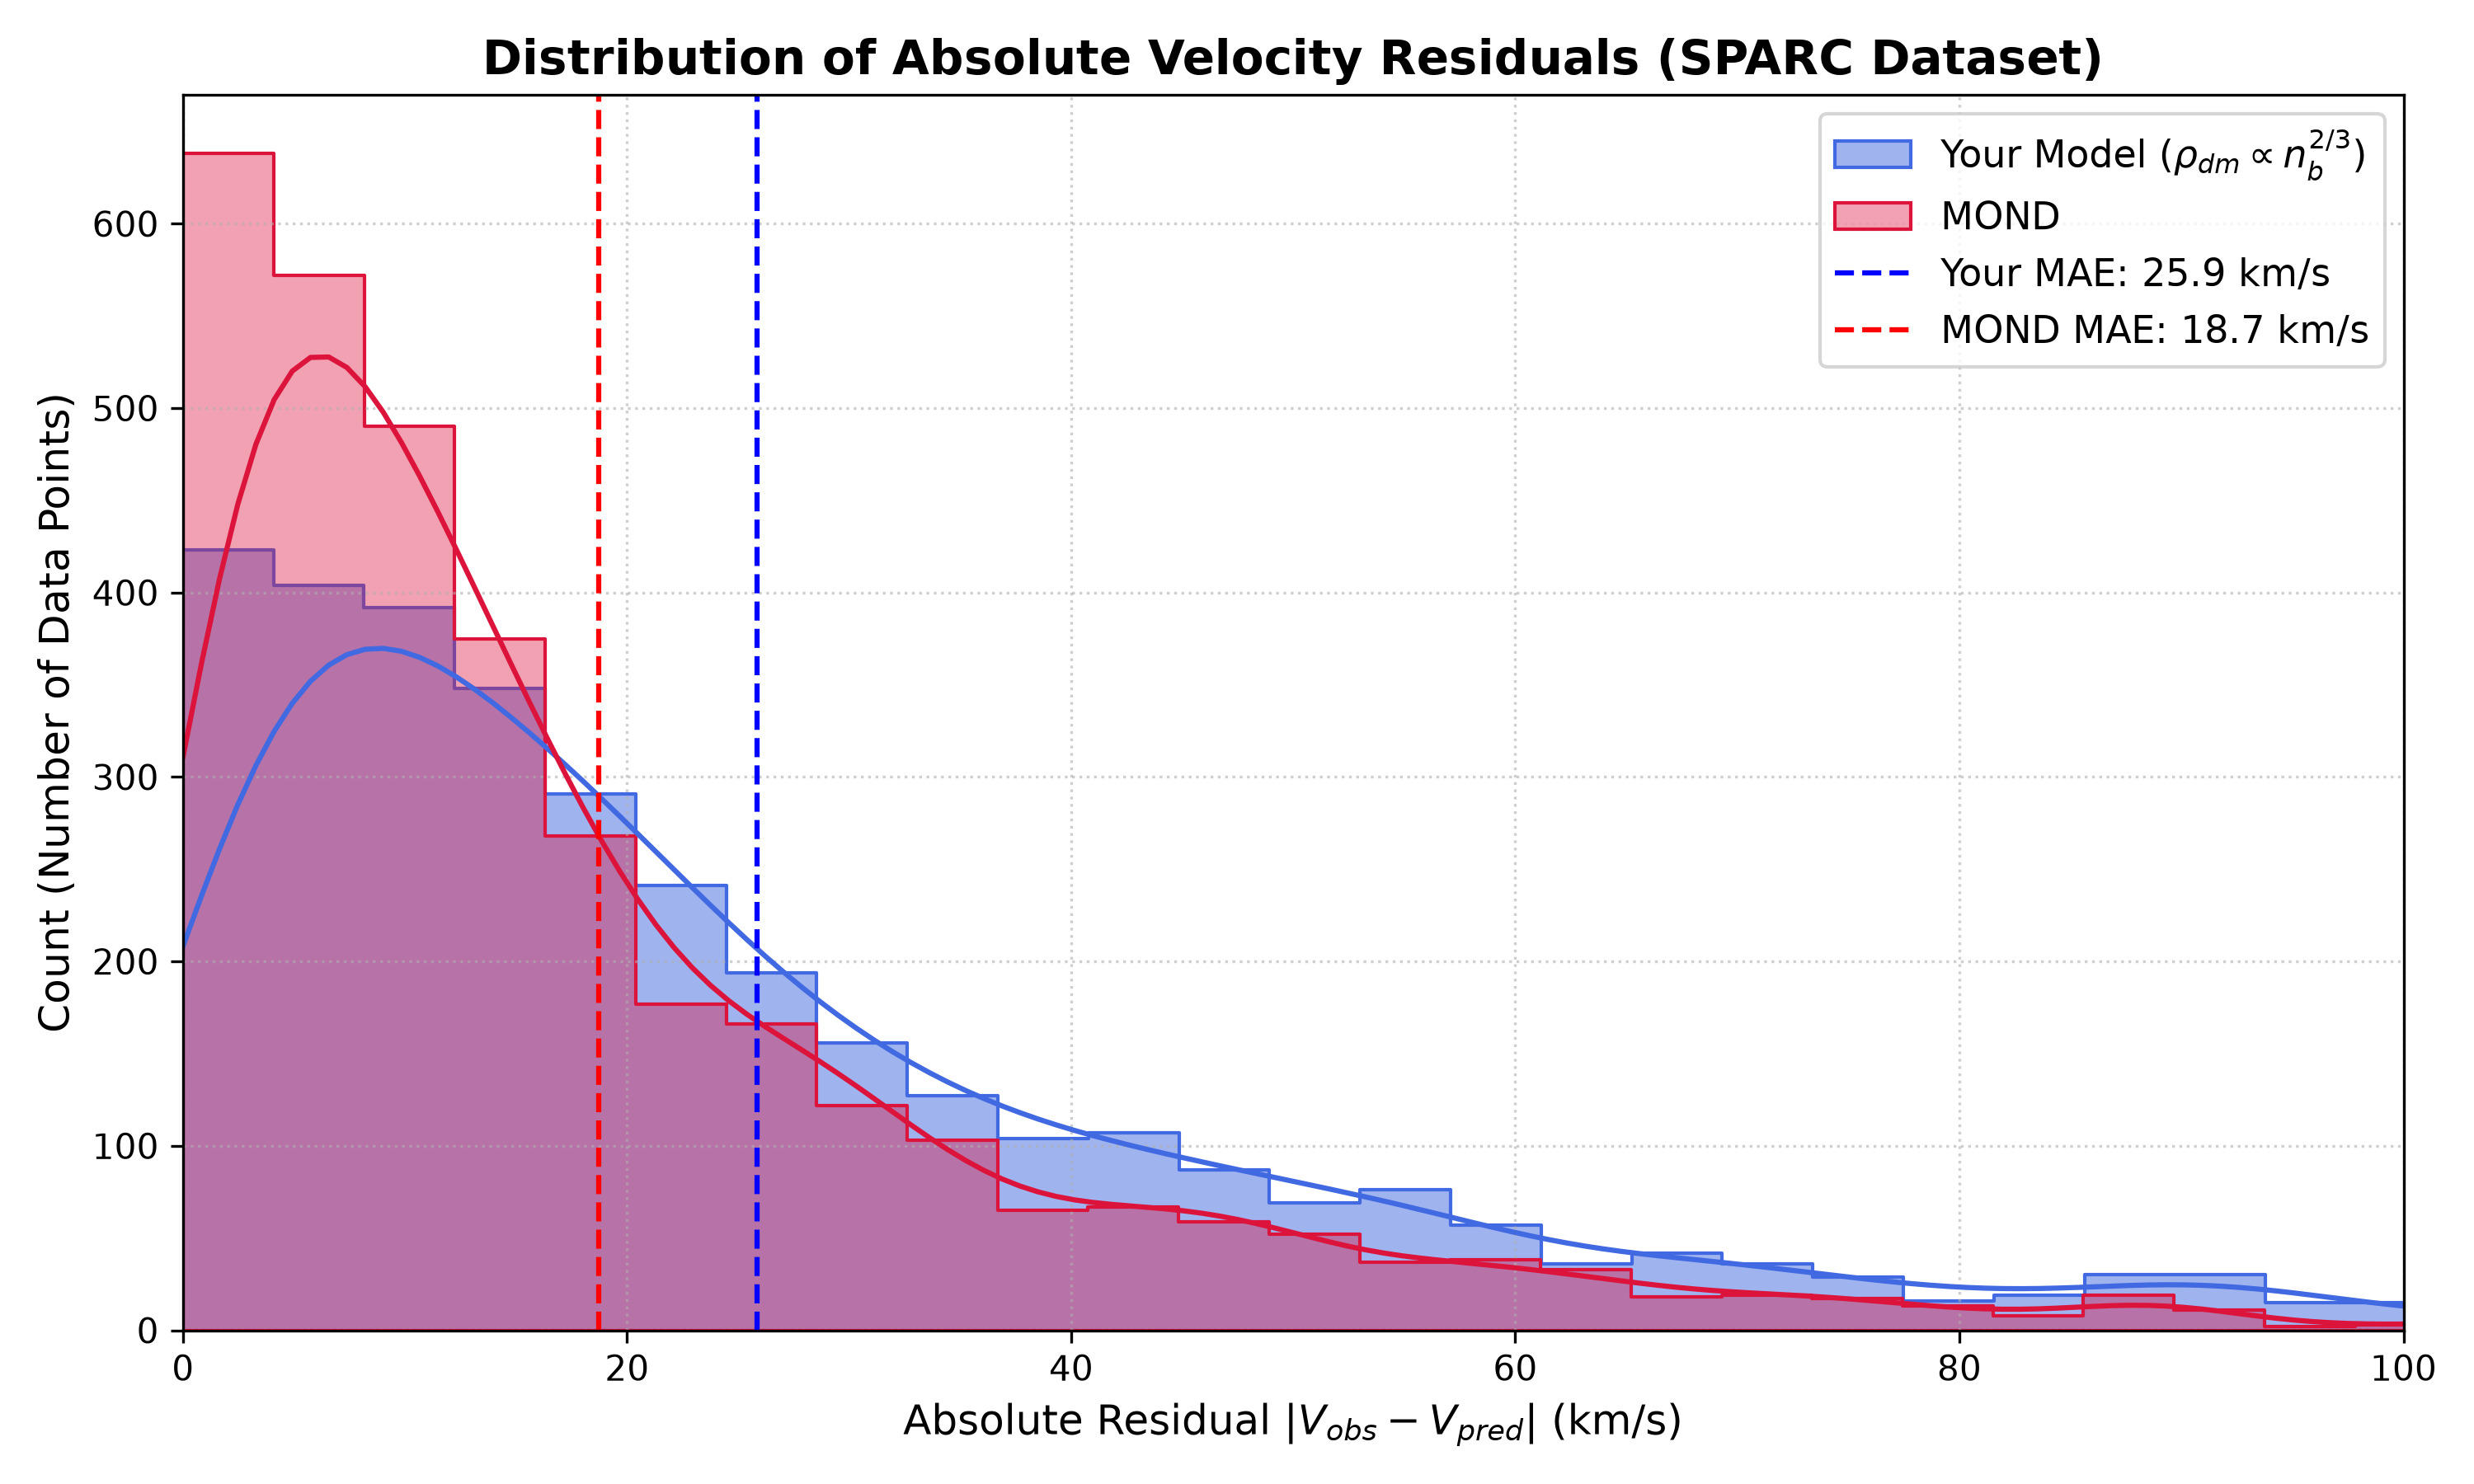
\includegraphics[width=0.48\textwidth]{absolute_residual_dist-power-59W.png} 
\end{center}
\caption{All 3319 SPARC data points are plotted. The acceleration implied by the observed velocity $V_{obs}$ is on the vertical axis, the x axis has the full acceleration from baryons + the dm field introduced in this paper. The red line is a Newtonian expectation, the blue line is a (log) straight line fit to the data. Also: velocity residuals.}
\end{figure}


\subsection{Model Results}
The global optimization of our one-parameter model across all SPARC observations, results in a MAE of 26~km/s. The MOND framework as implemented here scores ($\text{MAE} = 19\text{ km/s}$). Our model achieves a remarkably similar accuracy profile using only a single universal parameter, like MOND. But unlike MOND, our model does not require the local particles to 'know' the global acceleration parameter, rather, they just have to 'know' the density of the material they are in. 

\subsection{Model Variations}
We also ran the model by adding 175 more fitting parameters, allowing each galaxy fit to adjust the entire gas density up or down by up to a factor of 5. This resulted in an ($\text{MAE} = 17\text{ km/s}$). 

In several SPARC radial bins, central core gas densities are recorded as zero. To test sensitivity to this, we implemented a physically motivated observational detection floor of $0.45\text{ baryons/cm}^3$ for unrecorded or low gas densities. Enforcing this floor shifts the global MAE by a negligible fraction, but it does make the global fit line up with Newton extremely well. 

These two model variations were not used in any of the other discussions in this paper, full results for them and a few others are available online. 

\begin{figure}[ht!]
\centering
\label{fig:histogram}
\begin{center}
\framebox[0.45\textwidth]{\parbox{0.4\textwidth}{\centering \vspace{2cm} [Figure 1: Overlapping Histogram of Absolute Velocity Residuals for Both Models vs. MOND] \vspace{2cm}}}
\end{center}
\caption{Distribution of absolute velocity residuals $|V_{\text{obs}} - V_{\text{pred}}|$ evaluated across the 3,391 data points of the SPARC dataset. Vertical dashed lines point out the global MAEs.}
\end{figure}

\subsection{Core Dynamics and Distribution Tails}
An analysis of the absolute residual distributions reveals that MOND's localized advantage is concentrated almost entirely in a tight low-error spike between 0 and 15 km/s, corresponding to high-density inner galactic cores. This divergence is physically expected; our model evaluates dark mass generation based purely on the gas density profiles, which frequently drop or fluctuate in stellar-bulge dominated cores. Crucially, in the intermediate and long-range tails ($25\text{ to }100\text{ km/s}$) - representing the low-acceleration, outer-disk environments - the error distributions of our model and MOND track one another identically. This strongly implies that in the highly rarefied outer halo regime, our geometric density relation functions as a direct mathematical dual to MOND's physical behaviour, without requiring complex acceleration interpolations.

\begin{figure}[ht!]
\centering
\label{fig:radial_error}
\begin{center}
\framebox[0.45\textwidth]{\parbox{0.4\textwidth}{\centering \vspace{2cm} [Figure 2: Absolute Model Error vs. Distance from Galactic Center (Radius in kpc)] \vspace{2cm}}}
\end{center}
\caption{Moving average trend line showing absolute model errors as a function of radial distance from galactic centers, indicating where core fluctuations stabilize.}
\end{figure}

\section{Conclusion} \label{sec:conclusion}

In this paper, we have evaluated a universal, one-parameter empirical dark matter density profile defined by the geometric relation $\rho_{\text{dm}} = P/c^3 \cdot n_b^{2/3}$ against the complete SPARC database. By optimizing the global constant via robust Least Absolute Deviations (LAD) regression across 3,391 data points from 175 morphologically diverse galaxies, our model achieves a global Mean Absolute Error (MAE) of 26~km/s. This performance is comparable to the MOND framework ($\text{MAE} = 18.7\text{ km/s}$). Both frameworks use a single parameter to model DM across all galaxies.

The statistical parsimony of this model provides compelling evidence for a universal coupling between baryonic density and dark mass distribution. We demonstrate that the $2/3$ scaling law captures the observations of the dataset.  

An analysis of the absolute residual distributions reveals that while MOND maintains an advantage in dense, stellar-dominated galactic cores, the two models track one another identically across the low-acceleration, outer-disk environments. This suggests that in the highly rarefied, widely spaced gas structures of the outer halo, our geometric density relation functions as a direct mathematical dual to MOND's phenomenological behaviour.

By focusing strictly on a data-driven, observational approach, this work side-steps the unconstrained parameter space of particle physics models that have remained undetected across decades of microphysical searches. We do not propose a specific microphysical mechanism for the $2/3$ scaling law, nor do we speculate on the fundamental properties of a constituent particle. Instead, we present this universal relation as an empirical reality mandated by galactic kinematics. We leave it to the particle physics and theoretical communities to engineer a fundamental mechanism---whether rooted in environmental screening, field-baryon interactions, or quantum vacuum geometries---capable of reproducing the strict observational constraints demonstrated here.

\bibliographystyle{aasjournal}
\bibliography{bibtex_tom} % where bibtex_tom.bib file lives


\end{document}
